\chapter{Results and Analysis}\label{ch_results}

\section{Evaluation of Interface and Workflow}
Two major interface design iterations occurred in this project. The
first iteration was concerned with solely displaying the functionality
of the project and the second was a more refined version where care
was taken over usability and aesthetics. 

The initial design was demonstrated to the authors peer group where
functionality could be shown and valuable feedback received. This
feedback was used to improve the design and workflow, and was used to
create the final design of the project. 

\subsection{Initial Design}
\begin{wrapfigure}{R}{0.29\textwidth}
  \vspace{-40pt}
  \centering
  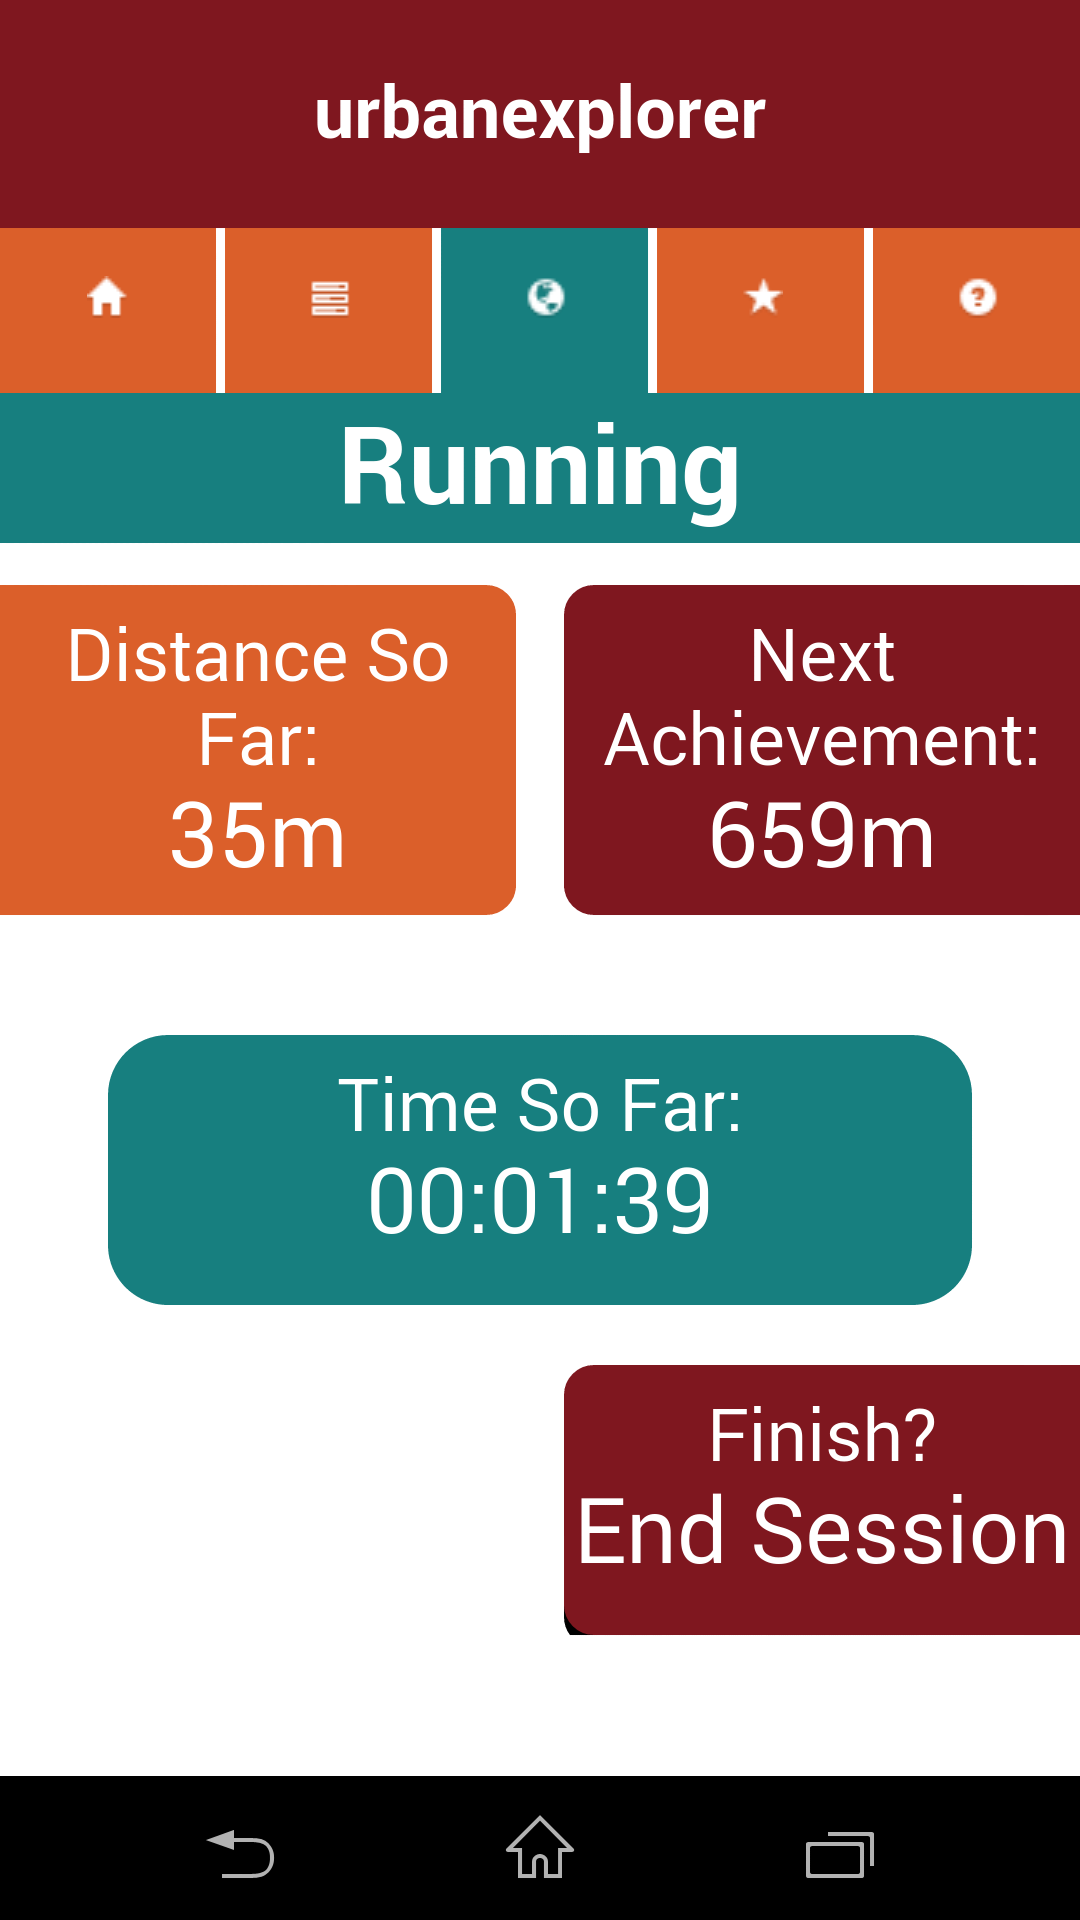
\includegraphics[width=0.29\textwidth]{images/init_design/run.png}
  \vspace{-20pt}
  \caption{Exercise Screen}
  \vspace{-25pt}
  \label{fig:init_run}
\end{wrapfigure}
When the initial design was formalised we did not have a solid idea of
what achievements would be in the context of this game. Therefore the
concept of an achievement does not feature predominantly in this
design iteration. 

Figure \ref{fig:init_run} shows the screen displayed when a user is
exercising. This screen is the key part of the application and was
given the most scrutiny. This design iteration had the same
functionality that the final design has in terms of the underlying
behaviour but users were quick to bring attention to the lack of
information displayed. The time and distance a user has travelled in
this exercise session (\emph{Distance So Far} and \emph{Time So Far})
and the distance until the next stage is completed (\emph{Next
  Achievement}) are displayed but there is no indication as to how far
along a route a user has progressed, or their overall time spent on
the route so far.  

It was recommended that by reducing the white space between elements
in the application we could easily include more information that was
relevant to the exercise session. One user indicated that a pictorial
representation of how far they had travelled along a route would be
desirable to see. The user likened the representation to a \emph{Horse
  Racing Derby
  Game}\footnote{\url{http://www.funfairstalls.co.uk/horse-racing-derby-game/4577291897}}
where the you have to complete a task, say rolling a ball into a hole,
and this advances your towards your goal, moving the horse closer to
the finish line. In our problem domain the task would be travelling
outdoors and the goal would be completing this route. By easily
substituting the horse model for a little running person we could map
our domain straight onto the fairground amusement. 

This idea was semi-realised in the final design and will be discussed
further in the final design section (Section
\ref{sec:final_design}). It is important to note that a user was able
to comprehend the abstract nature of our gamification goals and
then interpret them in terms of a game they know and understand. A key
part of determining the validity of any form of gamification is
whether or not a user can understand what they need to do to
succeed. We discuss \emph{Routes} and \emph{Stages} in an abstract
sense as the user never physically travels along the path that the
\emph{Route} or \emph{Stage} defines, so it is rewarding to discover
that a user can make the connection between the abstract depiction and
a real world example.

Most users also commented on the colour scheme chosen for the first
design implementation. The garishness of the colours chosen was
apparent even before starting the first round of evaluation but
attention was drawn to what the colours can mean. Users commented that
using predominantly red colours may not be a good choice as the
application is intended to encourage, and red is not normally
associated with encouragement. An analysis by \citet{colours_red}
of how the colour red influences performance confirms this
speculation, however it is in a different problem domain. Future work
could be undertaken here to see if the findings of \citet{colours_red}
are consistent in an exercise domain. In our situation, the colour
scheme required attention so the decision was taken to respect the
literature and user feedback and change to a colour scheme that was
predominantly blue.

Users were asked what rewards they would want to receive as they
progress in this application. It was unanimously suggested that there
should be a reward for completing each \emph{Route} and most users
suggested that this reward should be time based. Not all users
requested that a reward should be given for completing a stages but
this was formally added after further discussion with the project
supervisor. 

\subsection{Final Design}
\label{sec:final_design}
Photos added to run screen to enhance \emph{story}


\section{Evaluation of Gamification}

\section{Evaluation of Platform}
PhoneGap has its merits as a mobile platform: you can achieve rapid
development cycles by taking advantage of strong JavaScript and CSS
frameworks, a ``write once, deploy anywhere'' strategy for multiple
platform development, and good integration with the phones native
functionality. However it is the details of the integration with the
native functionality that can leave wanting, especially for
geolocation information.

As is discussed in Section \ref{sec:location_mgmt}, we use the PhoneGap
provided location watch service to receive location information. It
was discovered during development that if the PhoneGap provided
location watch service could not obtain location information for any
reason then the request would fail silently. Geolocation information
cannot always be obtained due to factors outwith our control and so
failing silently does not allow the developer to enforce any form of
persistence when searching for location information. In the case that
we could not obtain location information it may be desirable to
immediately restart searching for location information to provide the
user with better quality of service, however other factors such as
power consumption then come in to effect which may be more detrimental
than a few missed waypoints. This would need to be further analysed in
future work to properly justify what the correct course of behaviour
is in this situation.

The biggest challenge with the PhoneGap platform was the inconsistency
within the documentation of the platform and also the instability of
the upgrade process. 

The PhoneGap platform is built of two main modules: the PhoneGap
module which is concerned with the developers interface to the phone,
and the Cordova module which is concerned with the device management.
There is disparity between platform installation documentation and the
plugin documentation (for the geolocation module
etc)\cite{phonegap_install, phonegap_cli,
  phonegap_geolocationAccessingFeature}. This inconsistency does not
fill the developer with confidence when the official recommendations
cannot agree on correct procedures. 

Considerable time was also lost during the first round of user
evaluation due to an undocumented step required during platform
updating. When an Android project is created a JAR is installed that
is responsible for interfacing with the device but updating the
PhoneGap project did not update this JAR. Since the JAR was not
updated it did not have new functionality that the project was
attempting to access and so was crashing the app. A solution was
eventually discovered on an unrelated thread\cite{pluginFix} and user
evaluation was able to continue. Time was unnecessarily lost over bad
documentation and wrong assumptions by the platform developers.

Other small issues like a provided build script to build a ``release''
version of the app for the Android Play Store builds a ``debug''
version instead, each time you build the app the version number and
release number are reset to their default values, an XML configuration
file for the app is ignored when searching for the main ``index.html''
file (root of the application), amongst others.

It is for these reasons that I could not recommend PhoneGap as a
platform that is viable for a production quality app. Until the
documentation and platform become more reliable and consistent the
benefits of cross platform development do not outweight the loss of
fidelity incurred by non native implementation.
